%****************************************************************************%
%* DIET Programmer's Guide - Annexe 1                                       *%
%*                                                                          *%
%*  Author(s):                                                              *%
%*    - Christophe PERA (christophe.pera@ens-lyon.fr)                       *%
%*                                                                          *%
%* $LICENSE$                                                                *%
%****************************************************************************%
%* $Id$
%* $Log$
%* Revision 1.1  2004/01/09 15:26:53  cpera
%* Add Annexe on Autotools.
%*
%****************************************************************************%


% This is detail description about autotools files
\appendix{Autotools in depth}

%\section{Autotools in depth}
This annexe describes autotools files. All its content is from "The Goat Book"
by Gary V. Vaughan, Ben Elliston, Tom Tromey and Ian Lance Taylor, published 
in October 2000 by New Riders publishing and freely available online at 
http://sources.redhat.com/autobook/autobook/autobook.html.

%\footnote{"GNU autoconf, automake and libtool" from Gary V. Vaughan, Ben Elliston, Tom Tromey and Ian Lance Taylor {\url{http://sources.redhat.com/autobook/autobook/autobook.html}}}

\section{bootstrapping}
Bootstrap.sh is a shell script calling :
\begin{enumerate}
\item{libtoolize}
\item{aclocal}
\item{autoheader}
\item{automake}
\item{autoconf}
\end{enumerate}

\subsection{aclocal}
The aclocal program creates the file `aclocal.m4' by combining stock installed
macros, programer defined macros and the contents of `acinclude.m4' to define all
of the macros required by `configure.in' in a single file. Aclocal was 
created as a fix for some missing functionality in Autoconf. Aclocal is a part of
automake package.

%\begin{figure}[h]
\begin{center}
\includegraphics[scale=.35]{fig/DiagrammeAclocal.eps}
\end{center}
%\label{fig:aclocal}
%\caption{Aclocal files}
%\end{figure}

\subsection{autoheader}
autoheader runs m4 over `configure.in', but with key macros defined differently
than when autoconf is executed, such that suitable cpp definitions are output
to "DIET\_config.h.in". It is a part of autoconf package.

\begin{center}
\includegraphics[scale=.35]{fig/DiagrammeAutoheader.ps}
\end{center}

\subsection{Automake and Libtoolize}
Automake\footnote{Automake {\url{http://www.gnu.org/software/automake/automake.html}}} 
will call libtoolize to generate some extra files if the macro 
'AC\_PROG\_LIBTOOL' is used in `configure.in'. If it is not present 
then automake will install `config.guess' and `config.sub' by itself.

libtoolize\footnote{Libtool {\url{http://www.gnu.org/software/libtool/libtool.html}}}
can also be run manually if desired. 
Automake will only run libtoolize automatically if `ltmain.sh' and `ltconfig' 
are missing. In DIET, we choose to call explicitly libtoolize before automake
in bootstrap.sh.

\begin{center}
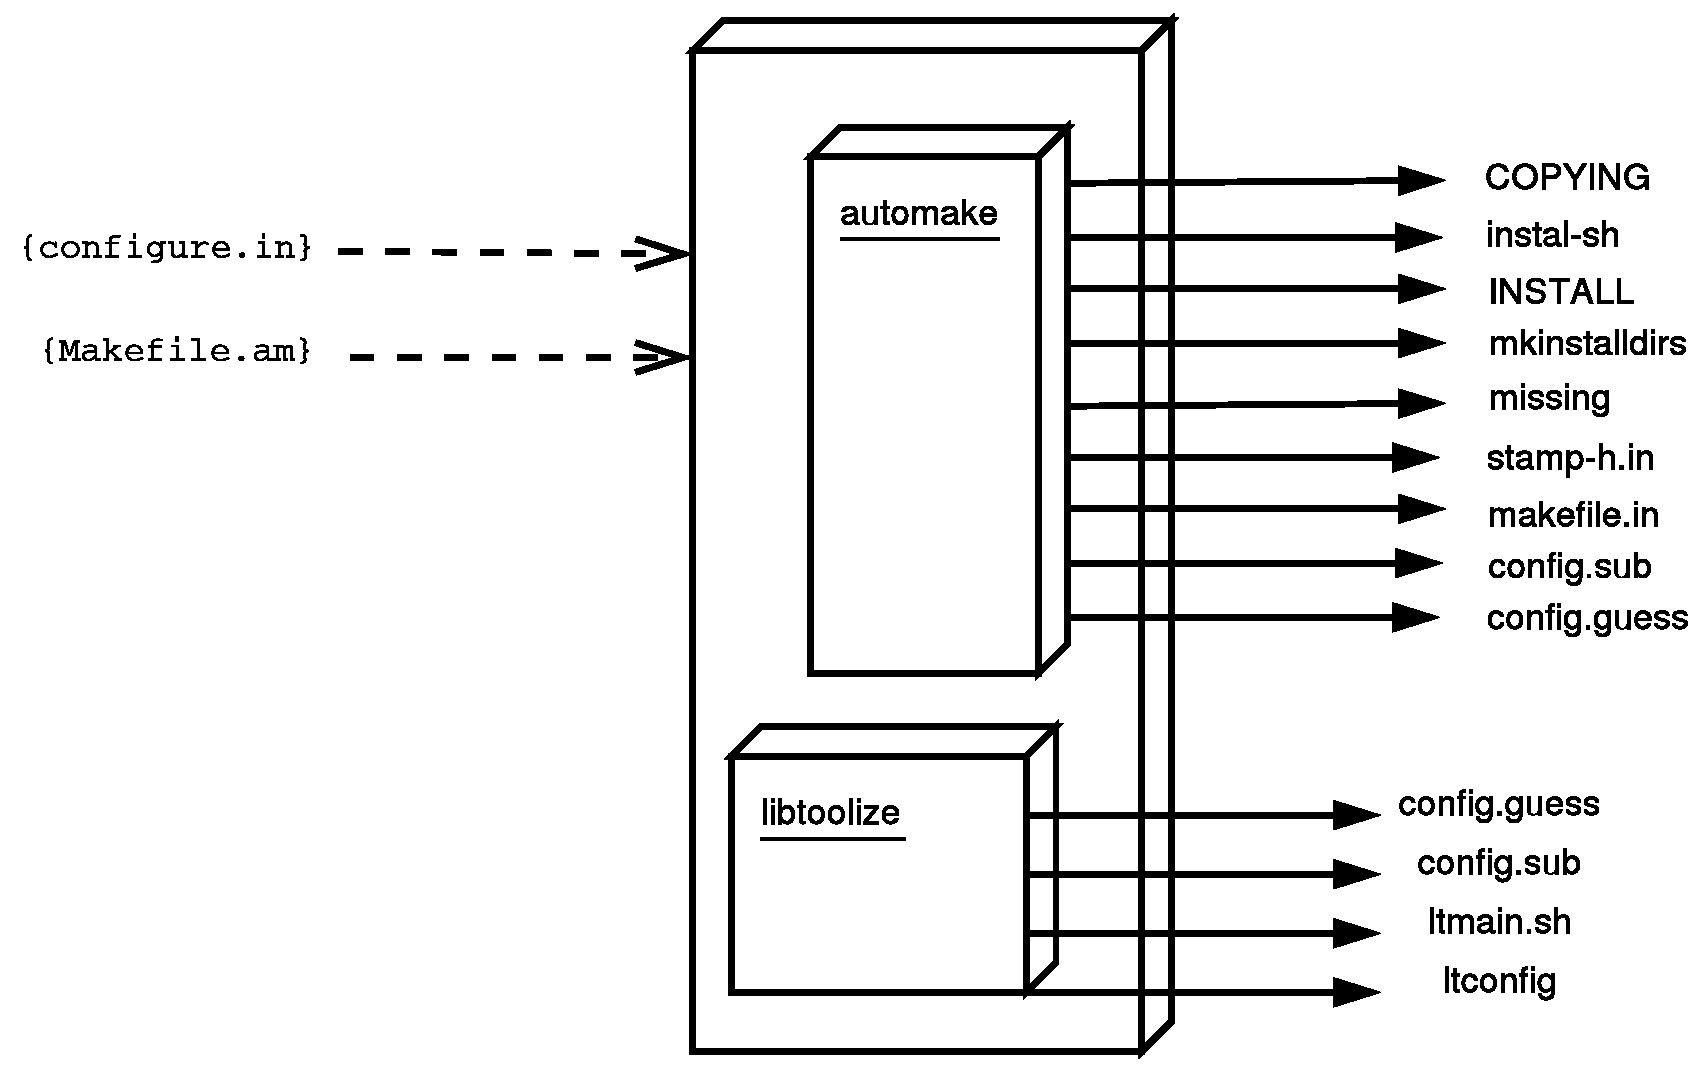
\includegraphics[scale=.35]{fig/DiagrammeAutomakeLibtoolize.ps}
\end{center}

The versions of `config.guess' and `config.sub' installed differ between 
releases of Automake and Libtool, and might be different depending on whether 
libtoolize is used to install them or not. Before releasing your own package 
you should get the latest versions of these files from ftp://ftp.gnu.org/gnu/config,
in case there have been changes since releases of the GNU Autotools.
Currently, DIET is developped with, at least, libtool 1.4.3, automake 1.7.3 and 
autoconf 2.57. Bootstraping and compiling may succeed with others previous autotools version
but it is not garanteed.
%\footnote{Automake {\url{http://www.gnu.org/software/automake/automake.html}}}
%\footnote{Libtool {\url{http://www.gnu.org/software/libtool/libtool.html}}}


\subsection{autoconf}
autoconf\footnote{Autoconf {\url{http://www.gnu.org/software/autoconf/}}} expands the m4 macros in `configure.in', using macro 
definitions from `aclocal.m4', to generate the configure script.
\begin{center}
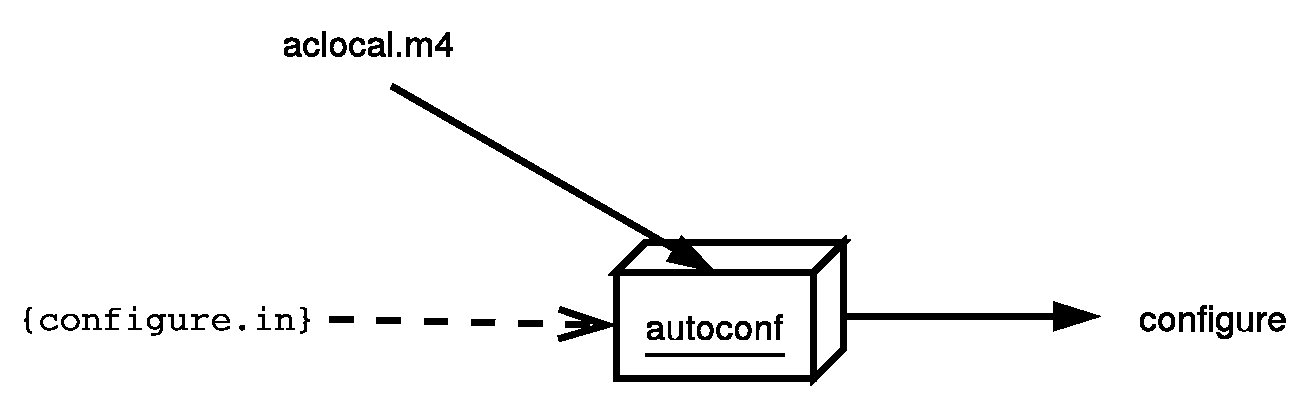
\includegraphics[scale=.35]{fig/DiagrammeAutoconf.ps}
\end{center}
%\footnote{Autoconf {\url{http://www.gnu.org/software/autoconf/}}}

\subsection{configure}
The purpose of the preceding processes was to create the input files necessary
for configure to run correctly. You would ship your project with the generated
script and the files in columns, other input and processes (except 
`config.cache'), but configure is designed to be run by the person installing
your package. Naturally, you will run it too while you develop your project,
but the files it produces are specific to your development machine, and are
not shipped with your package -- the person installing it later will run 
configure and generate output files specific to their own machine.

Running the configure script on the build host executes the various tests 
originally specified by the `configure.in' file, and then creates another script,
`config.status'. This new script generates the `DIET\_config.h' header file from 
`DIET\_config.h.in', and `Makefile's from the named `Makefile.in's. Once 
`config.status' has been created, it can be executed by itself to regenerate
files without rerunning all the tests. Additionally, `AC\_PROG\_LIBTOOL'
was used, so ltconfig is used to generate a libtool script. 

\begin{center}
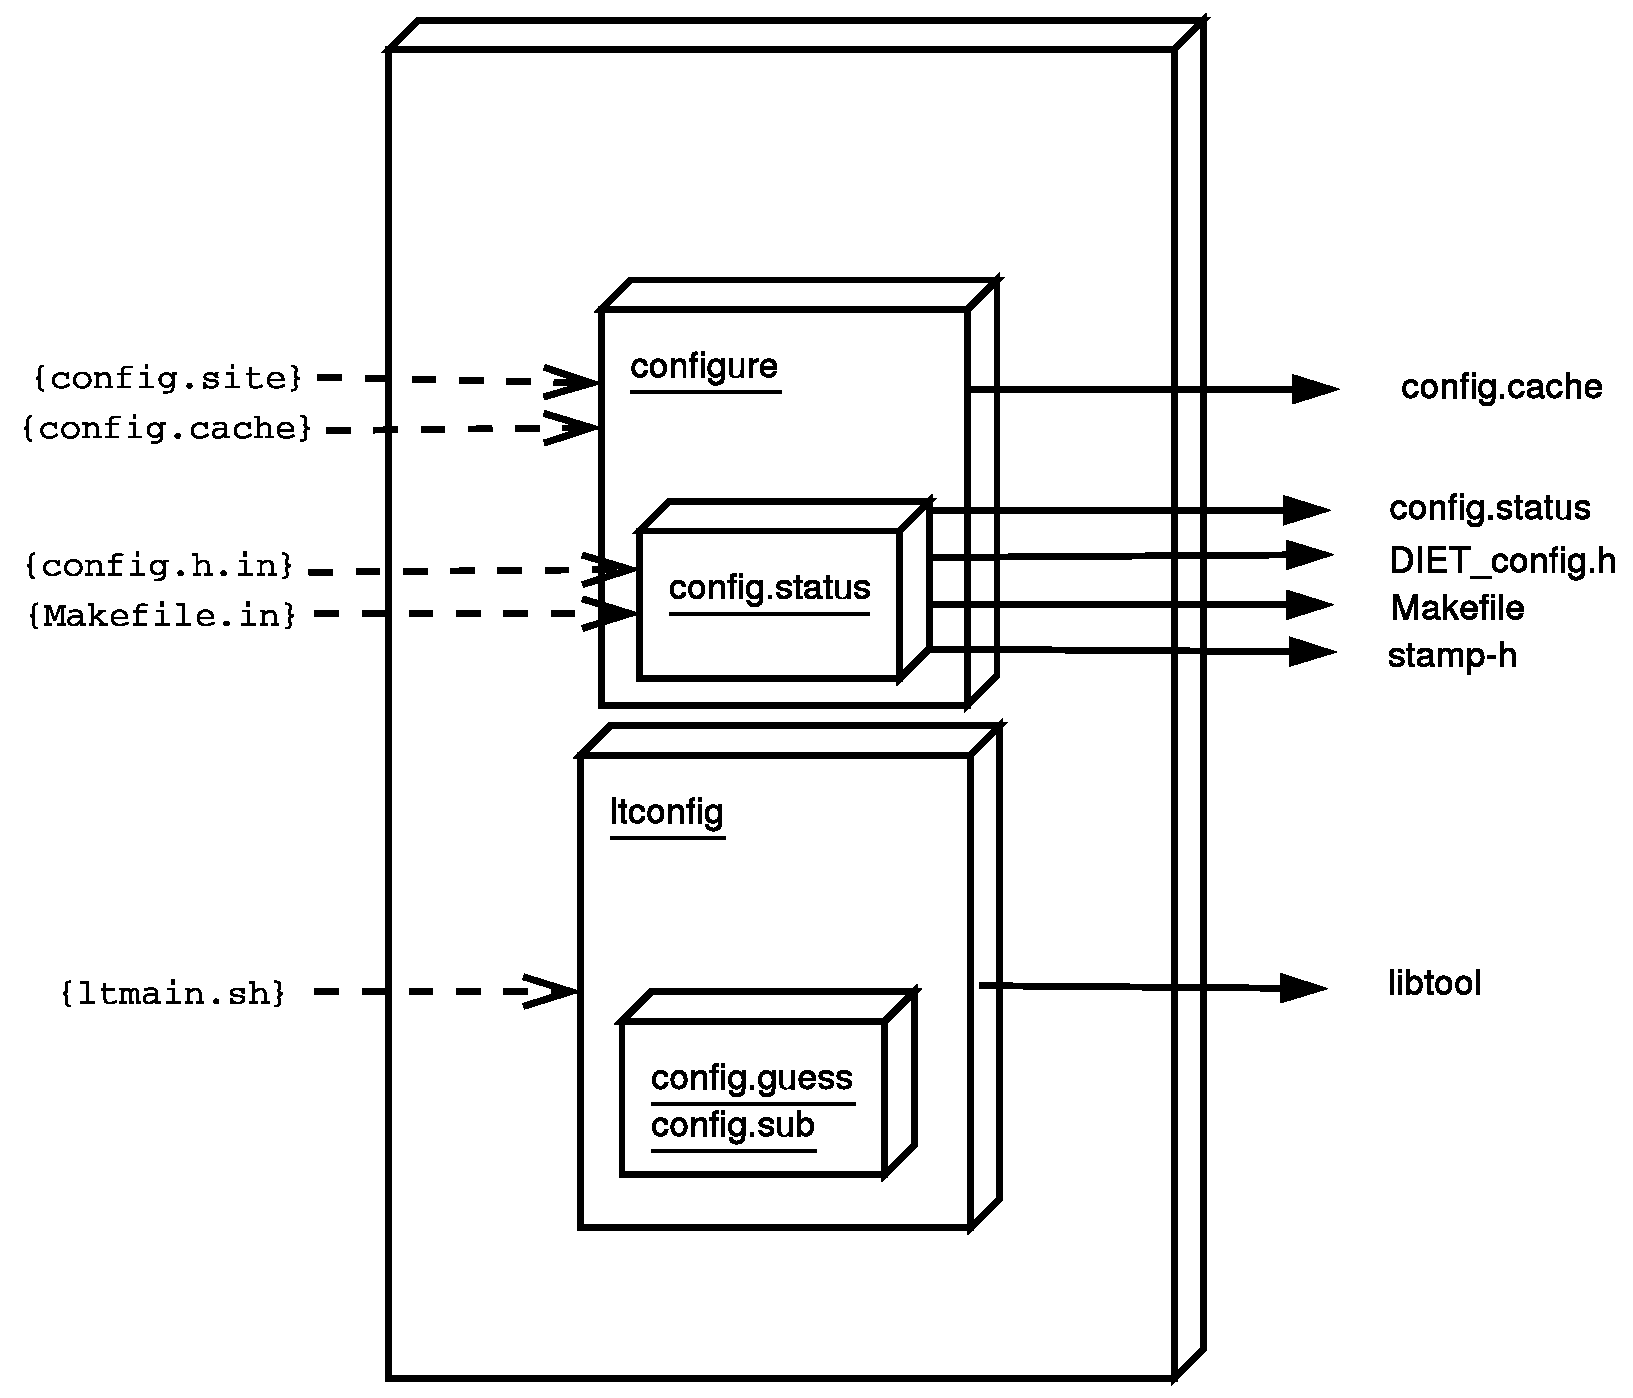
\includegraphics[scale=.35]{fig/DiagrammeConfigure.ps}
\end{center}

\section{CORBA and asynchronism}
Datas from the book "Advanced CORBA Programming with C++""
\footnote{"Advanced CORBA Programming with C++"  from Michi Henning, Steve Vinoski} and
from omniORB\footnote{OMNIORB {\url{http://www.uk.research.att.com/omniORB/}}}
and from TAO\footnote{TAO {\url{http://www.cs.wustl.edu/~schmidt/TAO.html}}
}

